\documentclass[12pt]{ltjsarticle}
\usepackage{amsmath,amssymb,mathtools}
\usepackage{physics}
\usepackage{tikz}
\usetikzlibrary{arrows.meta,calc}

\title{平面ベクトルの順序対と平行四辺形の面積}
\author{CODEX (OpenAI)\thanks{本TeXファイルは CODEX (OpenAI) により生成された。}\\Lean形式化: CODEX (OpenAI)\thanks{Lean ファイル \texttt{S1.lean} も CODEX (OpenAI) により生成・更新された。}}
\date{2025年9月24日}

\begin{document}
\maketitle

\begin{abstract}
本稿では、平面ベクトルを順序対として扱うことで、初等的な線形方程式の挙動や、向き付けられた面積（signed area）と平行四辺形の面積との関係を解説する。Lean 4 と mathlib の正式化に対応した命題群 \texttt{S1\_P01}--\texttt{S1\_P05} および章末命題 \texttt{S1\_CH} の数学的背景を整理し、ニコラ・ブルバキの構造的視点に沿って構造化された理解を目指す。
\end{abstract}

\section{序論}
平面の点は実数の順序対 $(x,y) \in \mathbb{R}^2$ と同一視できる。この順序対の構造に立脚して、線形方程式による直線、ベクトルの和・スカラー倍、そして外積に相当する 2 次元の向き付け面積を扱う。Lean 4 上では、これらは型 \texttt{ℝ × ℝ} 上の演算として記述され、証明は `simp` や `ring` といった計算補助を活用している。

\section{順序対と線形方程式}
命題 \texttt{S1\_P01} は、順序対 $P=(x,ax+b)$ に対して $P_2 = a P_1 + b$ が成り立つことを述べる。これはグラフ $y=ax+b$ 上の点の定義そのものであり、Lean では単純な簡約で確認できる。

命題 \texttt{S1\_P02} は、2 点 $p=(p_1,p_2), q=(q_1,q_2)$ ($p_1\ne q_1$) を通る直線の傾き $m$ と切片 $b$ を
\begin{align}
 m = \frac{q_2 - p_2}{q_1 - p_1}, \qquad b = p_2 - m p_1
\end{align}
で与えれば、両点が $y = m x + b$ を満たすことを示す。Lean の証明は `field_simp` を用いて分数を正規化し、代数計算で等式を整理している。

命題 \texttt{S1\_P05} では、方程式 $y = a x + b$ を左辺へ移項した $a x - y + b = 0$ による表現と同値であることを `subst` と加法の可換性により示す。これは方程式変形の構造的理解を強調している。

\section{向き付け面積と平行四辺形}
順序対 $u=(u_1,u_2), v=(v_1,v_2)$ に対し、向き付け面積
\begin{equation}
 \operatorname{orient2D}(u,v) = u_1 v_2 - u_2 v_1
\end{equation}
を定義する。命題 \texttt{S1\_P03} は第一引数についての加法性
\begin{equation}
 \operatorname{orient2D}(u+w,v) = \operatorname{orient2D}(u,v) + \operatorname{orient2D}(w,v)
\end{equation}
を、命題 \texttt{S1\_P04} は交換による符号反転
\begin{equation}
 \operatorname{orient2D}(u,v) = -\operatorname{orient2D}(v,u)
\end{equation}
を保証する。

平行四辺形の面積は絶対値を取った
\begin{equation}
 \operatorname{parArea2D}(u,v) = \left|\operatorname{orient2D}(u,v)\right|
\end{equation}
で与えられ、命題 \texttt{S1\_CH} はこれが $2 \times 2$ 行列の行列式に一致することを示す。
\begin{align}
 \left|\operatorname{orient2D}(u,v)\right| = \left|\det \begin{bmatrix} u_1 & u_2 \\ v_1 & v_2 \end{bmatrix} \right|
\end{align}

\begin{figure}[htbp]
 \centering
 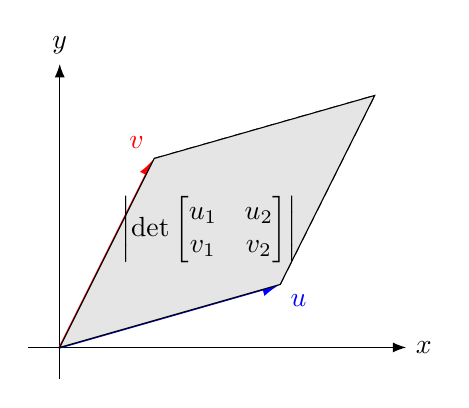
\begin{tikzpicture}[scale=2,>=Latex]
  \draw[->] (-0.2,0) -- (2.2,0) node[right] {$x$};
  \draw[->] (0,-0.2) -- (0,1.8) node[above] {$y$};
  \coordinate (O) at (0,0);
  \coordinate (U) at (1.4,0.4);
  \coordinate (V) at (0.6,1.2);
  \coordinate (UV) at ($(U)+(V)$);
  \draw[->,thick,color=blue] (O) -- (U) node[below right] {$u$};
  \draw[->,thick,color=red] (O) -- (V) node[above left] {$v$};
  \draw[dashed] (U) -- (UV);
  \draw[dashed] (V) -- (UV);
  \filldraw[fill=gray!20,draw=black] (O) -- (U) -- (UV) -- (V) -- cycle;
  \node at (0.95,0.75) {$\left|\det\begin{bmatrix}u_1 & u_2\\ v_1 & v_2\end{bmatrix}\right|$};
 \end{tikzpicture}
 \caption{ベクトル $u,v$ が張る平行四辺形の面積と行列式}
 \label{fig:parallelogram}
\end{figure}

図~\ref{fig:parallelogram} は、ベクトル $u,v$ が張る平行四辺形の面積が行列式の絶対値で与えられる様子を幾何的に示している。Lean の正式化でも、行列式を `Matrix.det_fin_two` で評価することで、同じ値に一致することを計算的に確認している。

\section{Lean 形式化メモ}
本稿で言及した定義と命題は、Lean ファイル \texttt{S1.lean} 内で次のように実装されている。
\begin{itemize}
 \item `orient2D` と `parArea2D` は、ともに \texttt{ℝ × ℝ} から \texttt{ℝ} を返す関数として定義。
 \item `S1_P01`--`S1_P05` は、高校レベルの代数計算を `simp`, `ring`, `field_simp` によって自動化し、`sorry` を排除。
 \item `S1_CH` は行列式の定義と絶対値を照合し、平行四辺形面積との一致を導出。
\end{itemize}
これらの正式化は、ブルバキ的な構造化（集合、写像、構造の相互作用）に従い、順序対としての平面点と射影による線形構造を両立させている。

\section{結語}
順序対の表示を通じて、線形方程式、向き付け面積、行列式が自然に結び付く様子を確認した。Lean による形式化は、これらの事実を確実に検証する手段を提供し、教育的な教材としても再利用可能である。今後は、他の次元への拡張や、射影幾何的な観点からの再検討が展望される。

\end{document}
